% !TeX root=../main.tex
\chapter{رویکرد گراف مبنا مکان‌یابی و کالیبراسیون به صورت همزمان}

\section{مقدمه}
همانطور که در فصل قبل ذکر شد، اگرچه حسگرهای فضای مفصل سریع و ارزان هستند، اما زمانی که از آنها برای اندازه‌گیری مقادیر مجری نهایی استفاده می‌شود، دقت مدل سینماتیکی برای تعیین دقت قابل دستیابی بسیار مهم است. علاوه بر این، در زمینه همجوشی و ترکیب اندازه‌گیری‌ها، هم‌ثبت کردن داده‌ها
\cite{hall1997introduction} 
 اولین گام اساسی است. به عبارت دیگر، حسگرها باید اندازه‌گیری‌های خود را در یک مختصات یکپارچه ارائه دهند. اهمیت هم‌ثبت به دلیل فرض اساسی نویز گاوسی با میانگین صفر در الگوریتم‌های ترکیب داده‌ها است.
 
 نکته قابل توجه دیگر برای ربات‌های آسان نصب، لزوم بی‌نیازی الگوریتم کالیبراسیون پیشنهادی به حسگرهای گران‌قیمت و یا حسگرهایی که نیاز به تعمیر و نگهداری سطح بالایی دارند، می‌باشد. علاوه بر این، فرآیند کالیبراسیون باید به اندازه‌ای ساده باشد که اجرای آن در مکان‌های مختلف آسان و سریع باشد. با اینکه کالیبراسیون موضوعی است که بسیاری از پژوهشگران به آن علاقه‌مند هستند، اما مفهوم بهره‌گیری از چندین حسگر برای بهبود نتایج کمتر مورد توجه قرار گرفته است.
 

از طرفی دیگر، افزون بر مفهوم و ضرورت کالیبراسیون در حوزه ربات‌ها، مکان‌یابی آنها نیز مورد توجه بسیاری قرار گرفته است. همانطور که پیش‌تر بیان شد، الگوریتم‌های بسیاری در راستای ترکیب حسگرها و همچنین کاهش زمان پردازش برای مکان‌یابی ربات به صورت زمان-واقعی در انواع دیگر ربات‌ها همچون ربات‌های خودران مورد استفاده قرار گرفته است.

در این فصل مروری بر روش‌های مرسوم کالیبراسیون و مکان‌یابی ربات‌ها خواهیم داشت. سپس نگاهی به معایب این روش‌ها خواهیم داشت و برای حل آن‌ها رویکردی را ارائه خواهیم داد که معایب این روش‌ها را برطرف کند. در نهایت با استفاده از این رویکرد، یک ربات کابلی را در نظر خواهیم گرفت و با اعمال رویکرد مطرح شده، نتایج کالیبراسیون و مکان‌یابی را به صورت همزمان ارائه خواهیم داد.

\section{روش های مرسوم مسئله کالیبراسیون} \label{seq:conventional_calibration}
به صورت کلی، انتظار می رود چنانچه به یک ربات در دنیای واقع یک ورودی مشخص اعمال شود، با اعمال همان ورودی به مدل پاسخی یکسان دریافت شود. با این حال همواره وجود نامعینی ها و عدم دقیق بودن پارامتر های مدل در واقعیت ما را از رسیدن به چنین پاسخی ایده آل باز می دارد. این نامعینی ها می تواند ناشی از تقریب هایی باشد که در مدل داریم و یا پدیده هایی که در مدل سازی مورد توجه کامل قرار نگرفته اند. جنس این نامعینی ها می تواند ریشه در سینماتیک ربات و یا دینامیک آن باشد. فرآیند کالیبراسیون می تواند این نامعینی ها را در جهتی کاهش دهد که پاسخ هایی که از مدل و ربات در پیاده سازی واقعی دریافت می کنیم، کاهش پیدا کند. آنچه در این کار مورد بررسی قرار گرفته است کالیبراسیون سینماتیکی می باشد. شکل \ref{fig:kinematicmodelerror} نمایش بلوکی از یک فرآیند کالیبراسیون سینماتیکی بنا بر تعریف بیان شده می باشد. همانطور که در این شکل مشاهده می شود آنچه به عنوان خطا در نظر گرفته می شود تفاوت مکان فضایی ربات است که ناشی از مدل سینماتیکی ربات (در اینجا سیتماتیک مستقیم) و ربات واقعی در فضای کاری ربات، با یک ورودی مشترک در فضای مفصلی آن می باشد. 

\begin{figure}[!t]
	\centering
	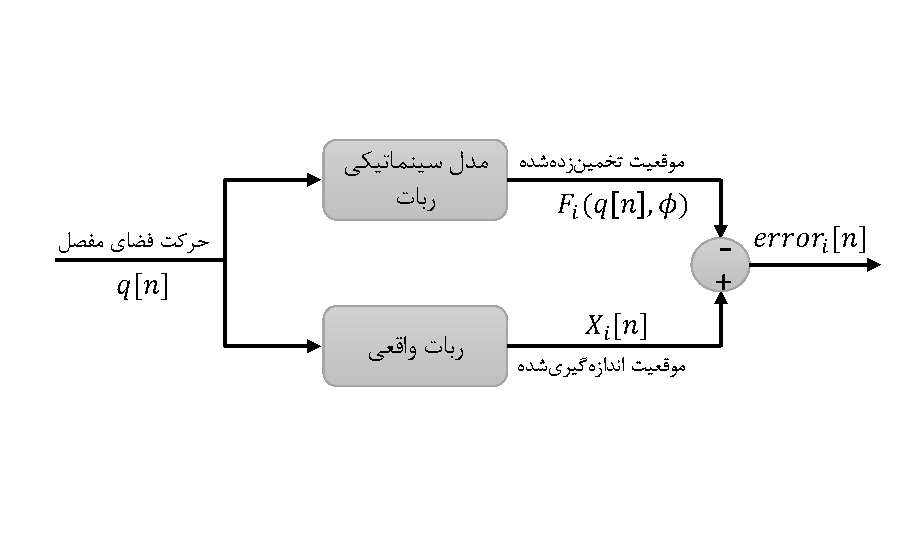
\includegraphics[width=0.8\linewidth, trim={0cm 2.2cm 0cm 2.2cm}, clip]{img/kinematic_model_error}
	\caption{دیاگرام کلی فرمول‌بندی یک مسئله کالیبراسیون}
	\label{fig:kinematicmodelerror}
\end{figure}


با نگاهی به آخرین تحقیقات بر روی مسئله کالیبراسیون ربات ها، ایجاد یک مسئله بهینه سازی غیرخطی و حل آن برای یافتن مقادیر دقیق این پارامتر های سینماتیکی و دینامیکی ربات مرسوم می باشد
\cite{elatta2004overview,ida2019automatic,ida2022identification,ida2021dynamics}.
مطابق این رویکرد های مروسم، برای ایجاد فرمول بندی مناسب مسئله مطرح شده در شکل \ref{fig:kinematicmodelerror} خواهیم داشت:

\begin{equation}\label{eq:optimization_equation_conventional}
	\tilde{\boldsymbol{\phi}} =  \arg\min_{\boldsymbol{\phi}} \sum_{n = 1 }^{N} \text{error}_i[n] = \arg\min_{\boldsymbol{\phi}} \sum_{n = 1}^{N} ||F_i(\boldsymbol{q}[n], \boldsymbol{\phi}) - X_i[n]||^2_{\Sigma}
\end{equation}

در این معادله، $\boldsymbol{\phi}$ بردار پارامتر های سینماتیکی و $\tilde{\boldsymbol{\phi}}$ تخمین آن است. علاوه بر این، $X_i[n]$، 
$iامین$
مقدار اندازه گیری شده توسط حسگر فضای کار ربات، و $\boldsymbol{q}[.]$ مقادیر اندازه گیری های متقابل حسگری در مفاصل می باشد. تابع مدل ربات $F[.]$ بیانگر مدل سینماتیک مستقیم ربات می باشد. تابع هزینه هدف، بر روی مجموعی از $N$ نمونه داده جمع آوری شده در فرآیند کالیبراسیون می باشد. افزون بر این، $\Sigma$ نیز بیانگر ماتریس کوواریانس اندازه گیری می باشد که به عنوان عامل نرمال سازی برای محاسبه هزینه عمل می کند. هر چه مقدار کوواریانس بیشتر باشد، میزان تاثیر گذاری خطای متقابل آن بر روی تابع هزینه کمتر خواهد بود. همچنین برای محاسبه نرم روش های زیادی ارائه شده است که آنچه بیشتر مورد استفاده قرار می گیرد نرم های هابر 
\footnote{\lr{Huber norms}}
می باشد
\cite{chang2015huber}.
معادله بهینه سازی غیر خطی بیان شده در 
\ref{eq:optimization_equation_conventional}
می تواند با روش های بازگشتی الگوریتم های غیر خطی حداقل مربعات
\footnote{\lr{Least-Square}}
همچون  لونبرگ-مارکوارت
\footnote{\lr{Levenberg Marquardt (LM)}}
و یا روش های گاوس-نیوتون
\footnote{\lr{Gauss-Newton(GN)}}
می باشد
\cite{dellart_robot_perception}.

با نگاهی دیگر به دیاگرام مطرح شده در 
\ref{fig:kinematicmodelerror}
و همچنین معادله 
\ref{eq:optimization_equation_conventional}،
مشاهده می‌شود که افزایش دقت اندازه‌گیری و همچنین برآورده کردن تمامی قیود مدل می‌تواند منجر به بهبود نتیجه کالیبراسیون شود. به منظور دستیابی به این هدف، رویکردهایی همچون ترکیب چندین حسگر و یا افزودن قیود جدید که از ساختار هندسی ربات استخراج می‌شود، معرفی می‌شوند. ترکیب این حسگرها باید به گونه‌ای باشد که علاوه بر کاهش خطای نهایی کالیبراسیون، خروج هر کدام از حسگرها منجر به توقف فرآیند کالیبراسیون نشود. همچنین واضح است که افزودن این قیود می‌تواند منجر به حل پیچیده‌تری از مسئله شود. در ادامه، نگاهی به فرمول‌بندی مسئله کالیبراسیون با در نظر گرفتن این ترکیب‌ها خواهیم داشت.

\subsection{ترکیب حسگر ها}
در معادله 
\ref{eq:optimization_equation_conventional}،
زیرنویس 
$i$
بیانگر وجود یک حسگر و خطایی که از مقادیر اندازه گیری حسگر در هر نمونه بوده می باشد. فرمول بندی ساختاری که به صورت همزمان از چندین حسگر در راستای ایجاد تابع هزینه استفاده نماید می تواند به صورت زیر تعریف شود:
\begin{equation}\label{eq:optimization_equation_conventional_multi_sensor}
	\tilde{\boldsymbol{\phi}} =  \arg\min_{\boldsymbol{\phi}} \sum_{n = 1 }^{N} \sum_{n = 1 }^{M} W_i~\text{error}_i[n] 
\end{equation}
در این معادله 
$W_i$
ها یک پارامتر وزن برای ترکیب چندین منبع اطلاعاتی با توجه به میزان کیفیت و اهمیت آنها می باشد.


\subsection{ترکیب شبه اندازه گیری ها}
اندازه گیری های حسگری تنها منبع اطلاعات برای حل مسئله نیستند. ساختار ربات و توحه به هندسه آن برای حل مسئله تعریف شده می تواند مفید واقع شود. برای مثال فاصله های بین برخی از نقاط می تواند با توجه به ساختار ربات می توانند ویژگی هایی نسبی و یا مطلق داشته باشند. این اطلاعات با عنوان داده های شبه اندازه گیری شناخته می شوند. این دسته از اطلاعات که از قبل مشخص هستند، می توانند به صورت قیود به مسئله اضافه شوند. بنابراین مسئله کلی بهینه سازی کالیبراسیون
\ref{eq:optimization_equation_conventional_multi_sensor}
در حضور این قیود به صورت زیر باز نویسی می شود. 
\begin{equation}
	\begin{aligned} \label{eq:optimization_equation_conventional_multi_sensor_measurement}
		&\tilde{\boldsymbol{\phi}} =  \arg\min_{\boldsymbol{\phi}} \sum_{n = 1 }^{N} \sum_{n = 1 }^{M} W_i~\text{error}_i[n] \\
		\quad &g_j(\boldsymbol{\phi}) = 0 \quad where \quad j = 1, \ldots, K
	\end{aligned}
\end{equation}
که در اینجا
$g_j(\boldsymbol{\phi}) = 0$ 
قیود هندسی معلوم بر روی پارامترهای سینماتیکی ربات می باشند.

\section{روش‌های مرسوم مسئله مکان‌یابی}
مکان‌یابی
\footnote{Localization}
 ربات فرآیند تعیین مکان ربات نسبت به محیط اطراف آن می باشد. دانستن مکان دقیق ربات در محیط، پیش‌نیازی اساسی برای اتخاذ تصمیمات صحیح و حرکت های بعدی مؤثر است. بدون اطلاعات مکانی دقیق، ربات نمی‌تواند مسیریابی
\footnote{motion planing}
  و یا ردیابی
\footnote{trakcing}
مناسبی را داشته باشد و ممکن است با موانع برخورد کند یا مسیر بهینه‌ای را طی نکند
\cite{ahmad2013cooperative}.
 علاوه بر این، سیستم‌های کنترلی ربات‌ها نیازمند اطلاعات دقیق و لحظه‌ای از مکان و جهت‌گیری ربات هستند تا بتوانند فرمان‌های مناسب را صادر کنند. بدون داده‌های دقیق مکانی، کنترلرها نمی‌توانند حرکات دقیقی را تولید کنند که منجر به عملکرد نامناسب و ناپایداری ربات می‌شود
\cite{guibas1997robot}.
فرآیند کالیبراسیون ربات که در بخش 
\ref{seq:conventional_calibration}
مورد بررسی قرار گرفت نیز یازمند داشتن اطلاعات دقیق از مکان ربات است. با داشتن داده‌های مکانی دقیق، می‌توان خطاهای سیستماتیک را شناسایی و تصحیح کرد و به این ترتیب دقت و کارایی ربات را بهبود بخشید. این امر به ویژه در ربات‌هایی که نیاز به انجام وظایف حساس و دقیق دارند، حیاتی است. 

مکان‌یابی دقیق ربات باعث کاهش عدم قطعیت در تصمیم‌گیری‌ها و عملیات ربات می‌شود. این امر نه تنها به افزایش اعتمادپذیری ربات در انجام وظایف محوله منجر می‌شود، بلکه احتمال بروز خطاها و حوادث ناشی از اشتباهات مکانی را نیز کاهش می‌دهد. همچنین در سیستم‌هایی که شامل چندین ربات هستند، اطلاعات دقیق مکانی هر ربات برای هماهنگی و همکاری بین ربات‌ها ضروری است. این اطلاعات به ربات‌ها کمک می‌کند تا از مکان یکدیگر آگاه باشند و بتوانند به صورت هماهنگ وظایف مشترک را انجام دهند. در این راستا توسعه و بهبود تکنیک‌های مکان‌یابی به منظور افزایش دقت و کارایی ربات‌ها، از اهمیت ویژه‌ای برخوردار است
\cite{aragues2011multi}.


روش های ارائه شده برای مکان‌یابی ربات را می توان به سه دسته اصلی مسافت پیمایی
\footnote{odometry}،
مکان‌یابی جهانی
\footnote{global localization}
و مکان یابی و نقشه یابی به صورت همزمان
\footnote{SLAM}
تقسیم کرد. این روش ها با توجه به نوع حسگرهای تعبیه شده بر روی ربات می تواند مورد استفاده قرار گیرد. ترکیب داده ها برای همانند آنچه در بخش
\ref{seq:conventional_calibration}
مورد توجه قرار گرفت، در مکان‌یابی و تخمین حالت ربات نیز می تواند نقش موثری را ایفا کند. حسگر های استفاده شده از نظر جنس داده ها و فرکانس داده برداری نیز می تواند متفاوت باشد که در ترکیب داده ها خصوصا زمانی که اجرای الگوریتم به صورت زمان واقعی می باشد، چالش برانگیز خواهد بود. طیف وسیعی از روش های مرسوم ارائه شده برای ترکیب داده ها در راستای تخمین حالت، رویکردهای بر مبنای فیلتر هستند. این روش ها که به رویکرهای آماری 
\footnote{stochastic}
نیز شناخته می شوند، در دو دهه اخیر فعالیت های زیادی را به خود اختصاص داده اند. پایه این روش ها بر قانون بیز
\footnote{Bayes law}
بنا نهاده شده است. مقاله
\cite{panigrahi2022localization} 
دسته بندی جامعی از روش های فیلتر مبنا برای تخمین مکان ارائه کرده است. از میان روش های بیان شده، کالمن فیلتر و فیلترهای ذرات
\footnote{particle filters}
به عنوان فراگیرترین رویکرد مورد استفاده قرار گرفته شده است. این فیلترها با استفاده از فرض مارکووی برای حالت ها و به کار گیری اطلاعات پیشین، تخمینی از حالت جدید ارائه می کنند. 

\section{رویکرد گراف مبنا برای حل مسئله کالیبراسیون و مکان‌یابی به صورت همزمان}
روش‌های مرسوم کالیبراسیون و مکان‌یابی ربات‌ها که تا به اینجا معرفی شده‌اند، فرمول‌بندی‌های مشخصی برای حل این دو مسئله ارائه داده‌اند. همانطور که در فصل قبل مشاهده شد، سادگی و سرعت بالای این روش‌ها باعث پیاده‌سازی گسترده آن‌ها گردیده است. با این حال، این روش‌ها دارای معایبی نیز هستند. 
اول اینکه برای هر مسئله کالیبراسیون و ربات، فرمول‌بندی مسئله باید از ابتدا توسعه داده شود. دوم اینکه  این روش‌ها از تنک بودن ذاتی مسئله‌ها برای سرعت بخشیدن به محاسبات استفاده نمی‌کنند.  بزرگ شدن و پیچیده شدن فرمول‌بندی این مسائل باعث می‌شود که از حل آن‌ها به صورت زمان واقعی فاصله گرفته شود.  همچنین، این روش‌ها برای حل مسائل غیرخطی نیاز به خطی‌سازی دارند که نه تنها به پیچیدگی‌های محاسباتی می‌افزاید، بلکه باعث کاهش دقت نیز می‌شود. 
سومین موضوع،  روش‌های مرسوم فیلتر مبنا از داده‌های جاری و لحظه‌ای استفاده می‌کنند که باعث می‌شود علاوه بر مشکلات در مدیریت داده‌هایی که با تأخیر به سیستم می‌رسند، نتوانند داده‌های تاریخی را به صورت کامل در یک مسئله بهینه‌سازی دسته‌ای وارد کنند. این مشکل در مسائل مکان‌یابی باعث ایجاد مشکلات جدی همچون لغزش
\footnote{drift}
و کاهش دقت تا حد قابل توجهی می‌شود. چهارمین عیب این روش‌ها، عدم انعطاف‌پذیری آن‌ها برای بسط دادن مسئله با افزودن قیود به سیستم یا داده‌های حسگری به آن است. با توجه به این معایب، روش‌های مرسوم ممکن است در برخی کاربردهای پیشرفته رباتیک کارایی لازم را نداشته باشند. 

در این فصل، رویکردی گراف مبنا برای حل مسئله کالیبراسیون و مکان‌یابی ربات بیان می‌گردد که با فرمول‌بندی یکپارچه، هر دو مسئله را به صورت همزمان در یک مسئله بهینه‌سازی حل می‌کند. ویژگی‌های ذاتی این رویکرد در حل این مسئله واحد به تمامی معایب مطرح شده در روش‌های مرسوم پاسخ می‌دهد و باعث ایجاد حلی کامل و قابل بسط می‌شود. این رویکرد گراف مبنا به دلیل استفاده از ساختارهای گرافی، قادر به مدیریت بهینه‌تر داده‌های مختلف است. با ادغام تمامی داده‌های تاریخی و جاری در یک مسئله بهینه‌سازی دسته‌ای، این روش از داده‌های ورودی به صورت کامل استفاده کرده و به مشکلات مدیریت داده‌های تأخیر دار و لحظه‌ای غلبه می‌کند. همچنین، به دلیل عدم نیاز به خطی‌سازی مکرر، دقت محاسبات افزایش یافته و پیچیدگی‌های محاسباتی کاهش می‌یابد. علاوه بر این، انعطاف‌پذیری بالای این رویکرد امکان افزودن قیود و داده‌های حسگری جدید را فراهم می‌کند، بدون آن که نیاز به بازتعریف کلی فرمول‌بندی باشد. این ویژگی‌ها، در کنار توانایی بهره‌گیری از تنک بودن ذاتی مسئله‌ها برای بهینه‌سازی محاسبات، این رویکرد گراف مبنا را به یک ابزار قدرتمند برای کالیبراسیون و مکان‌یابی ربات‌ها تبدیل می‌کند.

الگوریتم گراف مبنای استفاده شده برای این فرمول‌بندی در این پایان‌نامه، الگوریتم گراف عامل
\footnote{factor graph}
می‌باشد. در ادامه، ابتدا نگاهی بر ریاضیات مرتبط با الگوریتم گراف عامل خواهیم داشت و سپس گراف عامل یکپارچه‌ای را برای حل مسئله مطرح شده معرفی خواهیم کرد. گراف عاملی که در ادامه پیشنهاد خواهد شد، حلی سیستماتیک برای کنار هم قرار دادن بلوک‌های ساختاری (عامل‌ها) در راستای تعریف یک مسئله کالیبراسیون در کنار مسئله مکان‌یابی به صورت یکپارچه است، که قابلیت گسترش به حسگرهای بیشتر و قیود اضافی را نیز دارا می‌باشد. علاوه بر این، از آنجایی که پیاده‌سازی‌های منابع باز و بهینه‌سازی شده برای این روش وجود دارد، مسئله کالیبراسیون و مکان‌یابی همزمان مطرح شده می‌تواند بر روی سیستم‌های نهفته بر روی ربات نیز پیاده‌سازی گردد. در این پایان‌نامه برای پیاده‌سازی گراف عامل پیشنهاد داده شده، از کتابخانه GTSAM استفاده شده است. 

\subsection{بیان الگوریتم گراف عامل}
مسئله غیرخطی تعریف شده در 
\ref{eq:optimization_equation_conventional_multi_sensor_measurement}
می‌تواند به‌صورت یک مدل گرافی که متشکل از گره‌هایی است که بیانگر متغیرهای تصمیم‌گیری هستند و یال‌هایی که ارتباط بین قیود و این متغیرها را نشان می‌دهند، بیان شود. در جامعه رباتیک، گراف عامل نمونه‌ای از این بیان است. این گراف‌ها یک چارچوب قوی و قابل انطباق برای بیان مسائل متنوع از تخمین حالت
\footnote{state estimation}
 تا برنامه‌ریزی حرکت
\footnote{motion planning}
 ، ارائه می‌دهند.  این الگوریتم برای حل مسائل بهینه‌سازی که شامل متغیرهای مختلف و قیود پیچیده است، مناسب می‌باشد. یکی از روش‌های بیان این مدل، استفاده از نمودارهای دو بخشی
$\boldsymbol{F} = (\mathcal{U}, \mathcal{V}, \mathcal{E})$
است که  عامل‌ها 
$(\mathcal{U})$
با استفاده از یال‌ها
$(\mathcal{E})$
روابط و قیودی را بین گره‌ها 
$(\mathcal{V})$
 ایجاد می‌کنند. بدین ترتیب بخش اول، یعنی گره‌ها، نمایانگر متغیرهای ناشناخته یا پارامترهای مدل هستند که آنها را با
$\boldsymbol{\phi_i}$
نشان می‌دهیم. به عنوان مثال، در مسئله کالیبراسیون و مکان‌یابی، گره‌ها می‌توانند نمایانگر مکان‌های مختلف ربات یا پارامترهای کالیبراسیون باشند. همچنین بخش دوم، یعنی عامل‌ها، نشان‌دهنده قیود یا روابط بین متغیرها می‌باشد که آنها را با
$\psi_i$
نشان می‌دهیم. این قیود می‌توانند شامل معادلات غیرخطی یا روابط پیچیده‌ای باشند که باید در فرآیند بهینه‌سازی در نظر گرفته شوند. بدین ترتیب یک گراف عامل 
$\boldsymbol{F}$
بیان کننده نحوه ایجاد یک تابع انرژی کلی
$\boldsymbol{\psi}$
از تک تک اجزای سیستم می باشد:
\begin{equation} 
	\boldsymbol{\psi}(\boldsymbol{\phi}) = \prod_{i} \boldsymbol{\psi}_i(\boldsymbol{\phi}_i) 
\end{equation}
کمینه‌سازی لگاریتم تابع 
$\boldsymbol{\psi}(\boldsymbol{\phi})$
منجر به ایجاد یک مسئله غیرخطی معادل می‌شود که مسئله بهینه‌سازی مورد نظر را مشخص می‌کند.


\subsection{گراف عامل پیشنهادی برای کالیبراسیون و مکان یابی به صورت همزمان}
  
همانطور که بیان شد، استفاده از گراف‌های عامل در مکان‌یابی ربات‌ها مزایای متعددی دارد. یکی از مزایای اصلی این است که گراف عامل می‌تواند به طور مؤثری اطلاعات نامطمئن را مدیریت کرده و تخمین‌های دقیق‌تری ارائه دهد. همچنین، این روش به دلیل ساختار گرافی خود، قابلیت انعطاف‌پذیری و مقیاس‌پذیری بالایی دارد، به طوری که می‌توان به راحتی اندازه‌گیری‌های جدید را به گراف اضافه کرده و تخمین‌ها را به‌روزرسانی کرد. در مسئله‌ی مکان‌یابی ربات‌ها، هدف اصلی تخمین دقیق مکان و جهت ربات در محیط است. برای این منظور، از اطلاعات مختلفی مانند داده‌های حسگرها، اندازه‌گیری‌های فاصله و داده‌های اینرسی استفاده می‌شود. گراف عامل این اطلاعات را به شکلی یکپارچه و هماهنگ ترکیب می‌کند.

برای مدل‌سازی مسئله مکان‌یابی با گراف عامل، ابتدا باید متغیرهای حالت ربات و محدودیت‌های مرتبط با آنها تعریف شوند. متغیرهای حالت می‌توانند شامل مکان و جهت پنجه ربات در نقاط مختلف زمانی نسبت به یک چارچوب پایه مشخص باشند. برای تعریف این متغیرهای حالت در زمان $i$ با کمک ماتریس انتقال پنجه ربات در فضای
$SE(3)$
به صورت زیر خواهد بود:
\begin{equation} \label{eq:transformation matrix}
	\boldsymbol{X}_i = \begin{bmatrix}
							\mathbf{R}_i & \mathbf{t}_i \\
								0 & 1
				     	\end{bmatrix}
\end{equation}
که 
$\boldsymbol{X}_i^{4\times4}$
 بیانگر ماتریس انتقال شامل ماتریس چرخش 
$\mathbf{R}_i^{3\times3}$
 و بردار انتقال 
 $ \mathbf{t}_i^{3\times1}$ 
 نسبت به چارچوب پایه می‌باشد. علاوه بر تعیین چارچوب پایه در حل مسئله مکان‌یابی، محدودیت‌ها نیز می‌توانند
شامل اندازه‌گیری‌های حسگرهای متفاوت باشد. 
 ما در این فرمول بندی
 حسگر اندازه‌گیری‌های اینرسی
\footnote{IMU} 
 و یک حسگر فاصله‌پیمایی چشمی
\footnote{Visual Odometry}
را به عنوان داده‌های اندازه‌گیری سیستم با فرکانس‌های متفاوت در نظر می‌گیریم. 

شکل 
\ref{fig:localization}
نشان‌دهنده گراف عاملی است که برای حل مسئله مکان‌یابی با فرضیات در نظر گرفته شده می‌توان ارائه کرد. دایره‌ها نشان‌دهنده متغیرهای مسئله هستند که در اینجا مکان ربات می‌باشند و آن‌ها را با ماتریس
$\boldsymbol{X}_i$ 
در زمان $i$ نمایش می‌دهد. مربع‌های رنگی نشان‌دهنده محدودیت‌ها و داده‌های حسگری هستند که با گذر زمان به سیستم وارد می‌شوند و زنجیره مکان ربات را نیز امتداد می‌دهند. چارچوب پایه تعیین شده که می‌تواند نقطه شروع یا نقطه استراحت ربات باشد، توسط یک عامل واحد
\footnote{unary factor}
(در اینجا مربع قرمز رنگ)، مکان‌یابی ربات را مقید می‌کند. همچنین داده‌های حسگری با توجه به فرکانس داده‌برداری آن‌ها می‌توانند به صورت عامل‌های دودویی که بین دو یا چند متغیر قیدی را ایجاد می‌کنند، وارد مسئله شوند. در این گراف، عامل‌های مشخص شده با رنگ سبز نشان‌دهنده اندازه‌گیری‌های حسگر اینرسی و همچنین اطلاعات حسگر فاصله‌پیمایی چشمی با عامل‌هایی به رنگ آبی وارد مسئله می‌شوند. با توجه به نرخ اضافه شدن این اطلاعات به سیستم، می‌توان دریافت که فرکانس داده‌برداری از حسگر اینرسی دو برابر حسگر فاصله‌پیمایی است. 
\begin{figure}
	\centering
	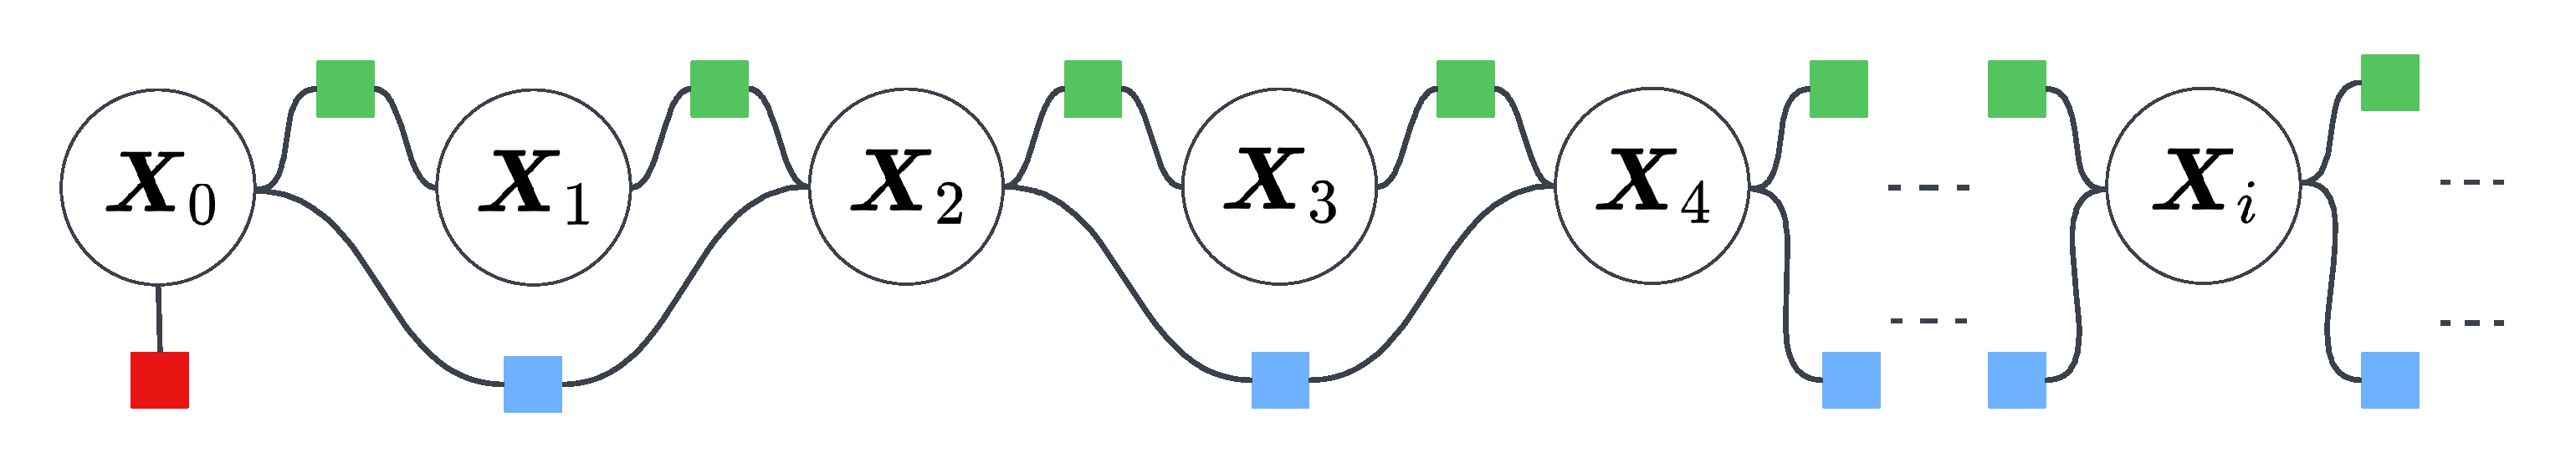
\includegraphics[width=0.7\linewidth]{img/Localization}
	\caption{گراف عامل پیشنهادی برای یک حل یک مسئله مکان‌یابی}
	\label{fig:localization}
\end{figure}

در این گراف، آنچه باعث حل یکپارچه و استفاده بهینه از تمامی اطلاعات مسئله می‌شود، زنجیره‌ای است که میان متغیرهای مسئله ایجاد شده است. با دریافت هر داده جدید از حسگر، یک متغیر مکان جدید برای ربات ایجاد می‌شود که حل مسئله بهینه‌سازی برای پیدا کردن این متغیر منجر به به‌روز رسانی تمامی گره‌ها به‌صورت یکجا می‌شود و این باعث ایجاد یک راه‌حل ارزشمند برای یک مسئله تنک می‌گردد. در این بخش، هدف تعریف پایه‌ای یک مسئله مکان‌یابی برای ربات است. گراف‌های متنوع و فرمول‌بندی‌شده برای اهداف خاص‌تر در
\cite{yang2022indoor}, 
\cite{song2021tightly}
و 
\cite{leitinger2017factor}
قابل مطالعه هستند. 

افزودن حسگرهای جدید با ایجاد گره‌های عامل با مدل نویزهای مناسب در فواصل زمانی منظم، می‌تواند نتیجه مکان‌یابی را بهبود بخشد. این ترکیب حسگرها می‌تواند در فواصل زمانی‌ای که حسگرها به‌دلیل شرایط محیطی از سیستم خارج می‌شوند، از توقف مکان‌یابی جلوگیری کند. به‌عنوان مثال، الگوریتم‌هایی که از داده‌های دوربین استفاده می‌کنند، زمانی که ویژگی‌های محیط برای پردازش تصاویر نامناسب است یا ربات وارد محدوده‌ای تاریک می‌شود، قادر به ارائه نتایج مناسبی نیستند. به عنوان نمونه‌ای دیگر، زمانی که سیستم مکان‌یابی جهانی
\footnote{GPS}
مورد استفاده قرار می‌گیرد، مکان‌هایی همچون تونل‌ها می‌توانند این سیستم جمع‌آوری داده را با مشکل مواجه کنند. بدین ترتیب، با خروج برخی از حسگرها مکان‌یابی با استفاده از داده‌های دیگر انجام می‌شود و با ورود مجدد حسگرها، نتایج رو به بهبود خواهند رفت. استفاده از این رویکرد محدود به نوع ربات و یا حسگرهای آن نبوده است.  
از ربات‌های خودران
\cite{wilbers2019localization}
تا ربات‌های پرنده
\cite{dai2022uav}
و یا ربات‌های جراح مورد استفاده در اتاق های عمل می توانند از این روش استفاده کنند. 


استفاده از گراف در مسئله مکان‌یابی برای ربات‌های چندعاملی می‌تواند کلیدی برای بهبود نتایج و فرمول‌بندی ساده‌تر باشد. سامانه آموزش جراحی چشم 
ARASH:ASiST 
در تیم آزمایشگاهی ارس توسعه یافته است
\cite{hassani2021kinematic}. این سامانه از دو دستگاه ربات مجزا برای تسهیل فرآیند آموزش جراحی تشکیل شده است. در این سامانه، ربات دوم باید حرکات ربات اول را دنبال کند تا آموزش جراحی با استفاده از این سامانه انجام پذیرد. پیدا کردن چارچوب این ربات‌ها در یک دستگاه مختصات می‌تواند یکی از ابزارهایی باشد که در پیاده‌سازی الگوریتم‌های متنوع کنترلی در فرآیند یادگیری مهارت مورد استفاده قرار گیرد. یکی از روش‌های پیشنهادی برای این هدف می‌تواند استفاده از گراف شکل 
\ref{fig:arashasistlocalization}
باشد. در این گراف، مکان‌یابی برای هر کدام از این ربات‌ها با به‌روز رسانی
$\boldsymbol{X}_{i}$
و
$\boldsymbol{X}_{i}^{'}$
برای هر یک از ربات‌ها به صورت مجزا، انجام می‌شود. هم‌چارچوب‌سازی این دو ربات می‌تواند توسط قیود عاملی که در اینجا با رنگ نارنجی نشان داده شده است، انجام شود. دیگر عامل‌ها با رنگ‌های مشخص شده همانند تعاریف بیان شده در شکل 
\ref{fig:localization}
می‌باشند. 

\begin{figure}
	\centering
	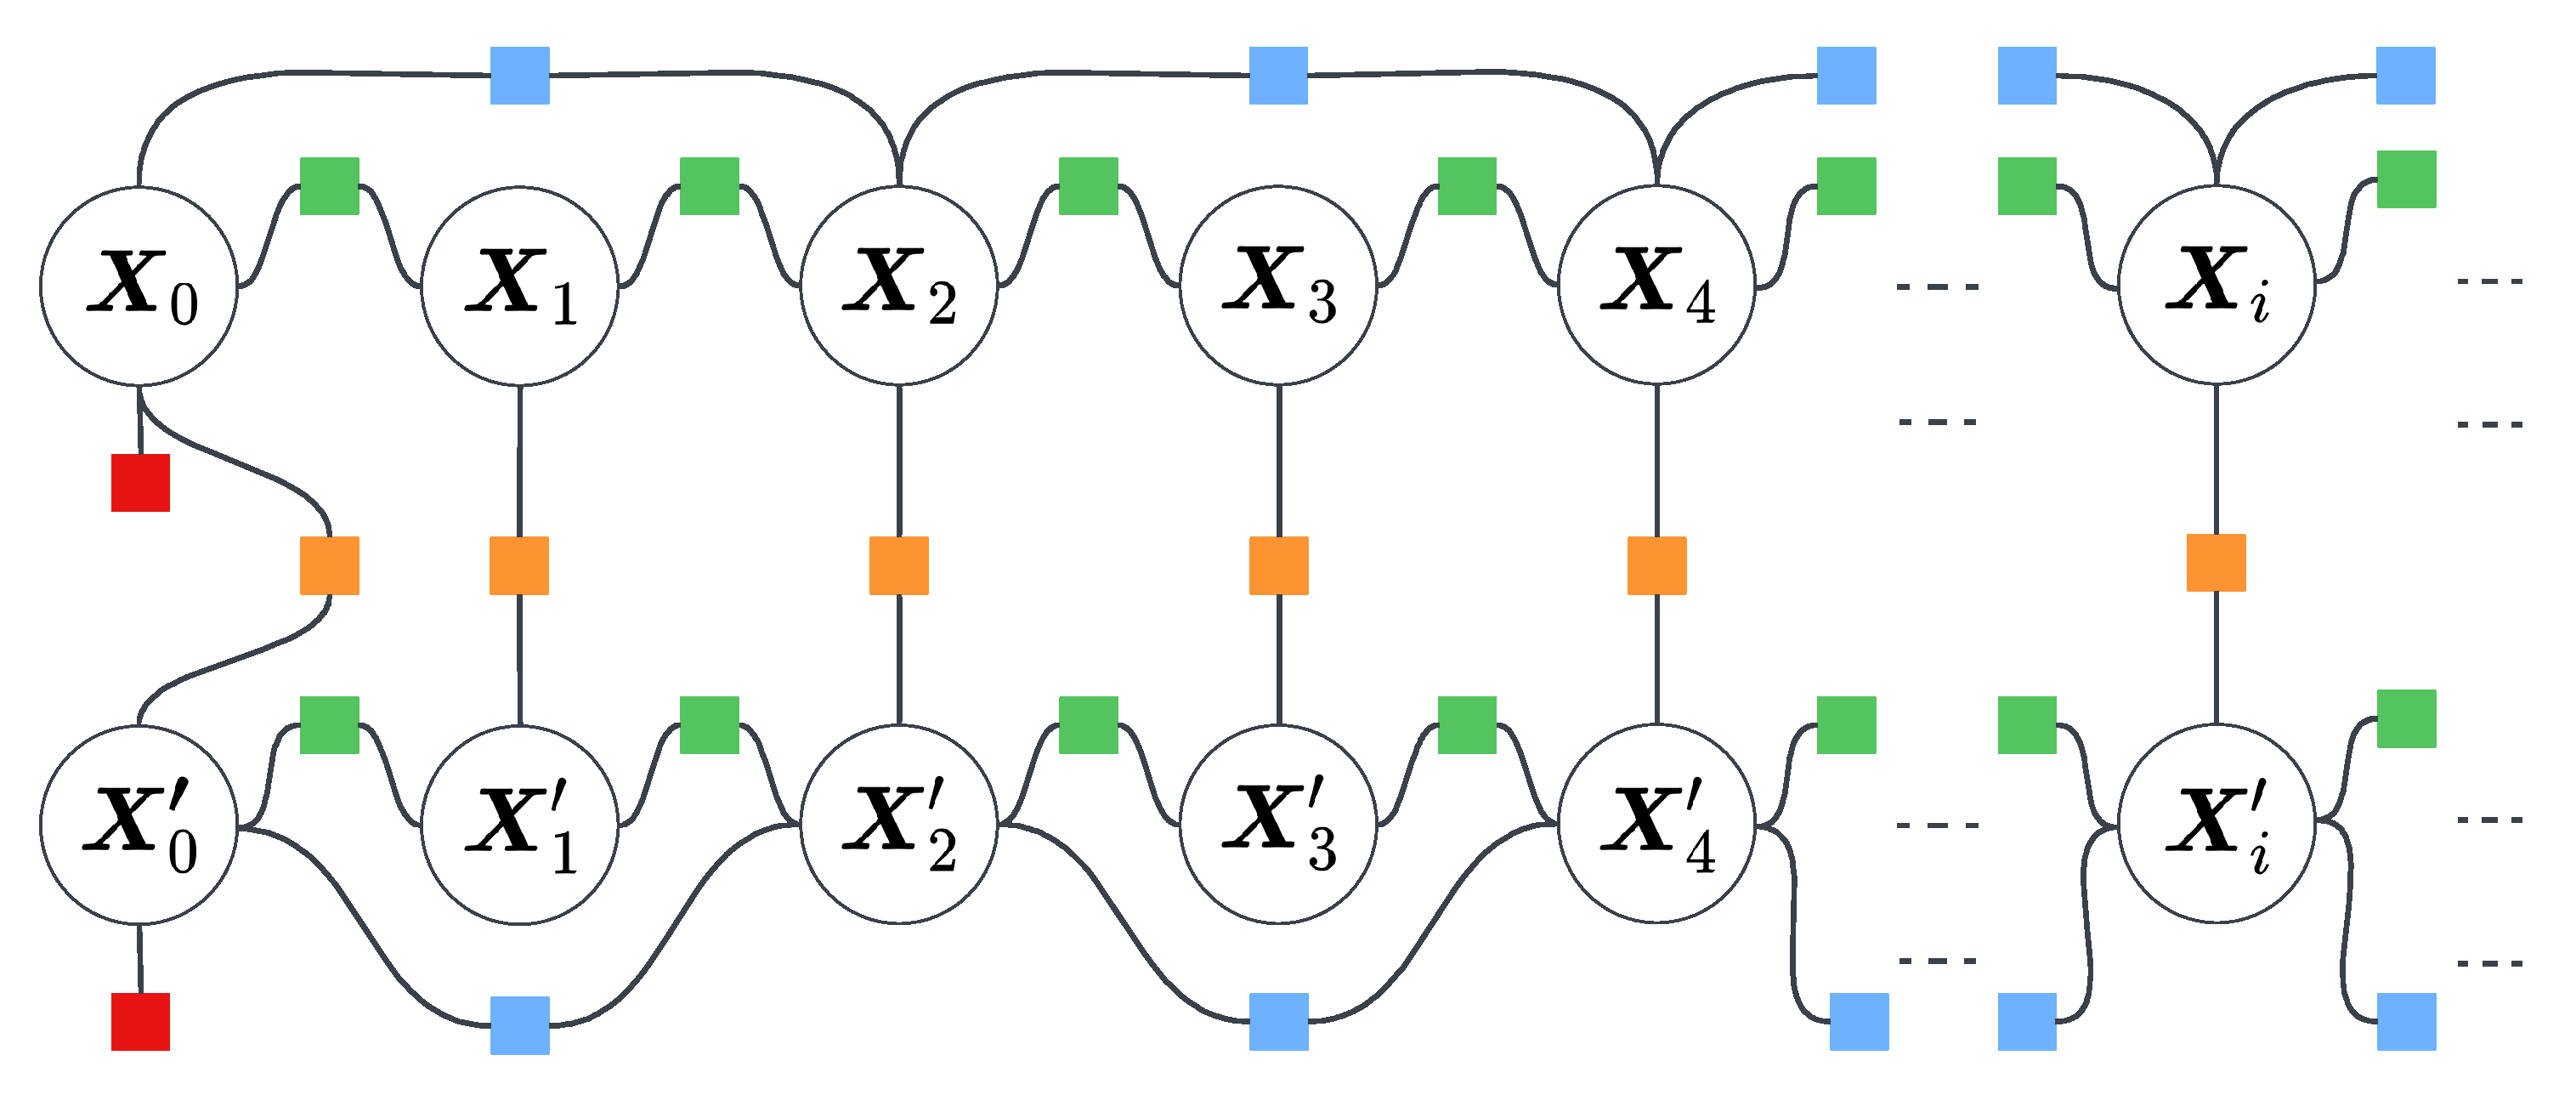
\includegraphics[width=0.7\linewidth]{img/Arash_Asist_localization}
	\caption{گراف عامل پیشنهادی برای یک حل یک مسئله مکان‌یابی ربات‌های چند عاملی}
	\label{fig:arashasistlocalization}
\end{figure}


آنچه تا بدین جای حل مسئله مشاهده شده است، توانایی بالای الگوریتم گراف عامل در ایجاد مسئله‌ای انعطاف‌پذیر بوده است. مقیدسازی این مسئله می‌تواند از قیود فضای کار ربات فراتر رفته و مسئله را در فضای مفصلی و ساختار سینماتیک ربات نیز مقید کند. وجود پارامترهای سینماتیکی در فرمول‌بندی می‌تواند با در نظر گرفتن آنها به‌عنوان متغیرهایی که همواره در ربات ثابت هستند یا متغیرهایی که با گذر زمان تغییر می‌کنند، به‌عنوان پارامترهای کالیبراسیون، مقادیر بهینه آنها را به‌دست آورد. به عبارتی، در حالی که مسئله مکان‌یابی در حال انجام است، مسئله کالیبراسیون نیز حل شود. همچنین اضافه شدن این قیود سینماتیکی می‌تواند مکان‌یابی ربات را بهبود بخشد.

مطابق فرمول‌بندی‌های مرسوم ارائه شده، معادلات سینماتیک نگاشت‌های غیرخطی بین فضای مفصل و فضای کار ربات ایجاد می‌شوند. بدین ترتیب:
\begin{equation} \label{eq:IK_FK_genral_equations}
	\boldsymbol{X} = FK(\boldsymbol{q}, \boldsymbol{\phi}), ~~ \boldsymbol{q} = IK(\boldsymbol{X}, \boldsymbol{\phi})
\end{equation}
که
$\boldsymbol{X}$
مکان ربات در فضای کار و
$\boldsymbol{q}$
بردار مقدار زاویه‌ای/طولی مفصل‌های ربات هستند. در این معادله
$\boldsymbol{\phi}$
بردار پارامترهای سینماتیکی ربات است که به هندسه ساختاری ربات مربوط می‌شود.

در ادامه، با فرض آنکه ربات مسیری تصادفی را در فضای کاری خود طی می‌کند و همچنین داده‌های سنسوری در هر دو فضای معرفی شده در حال جمع‌آوری هستند، قصد داریم گراف
\ref{fig:localization}
را به گونه‌ای بسط دهیم که کالیبراسیون سینماتیکی ربات در کنار مکان‌یابی در یک گراف یکپارچه حل شود. برای این کار از قیود سینماتیکی
\ref{eq:IK_FK_genral_equations}
استفاده کرده و آنها را به‌صورت عامل به مسئله می‌افزاییم. ابتدا فرض کالیبراسیون را بر ثابت بودن پارامترهای سینماتیکی و عدم تغییر آنها در طول زمان می‌گذاریم. شکل
\ref{fig:kinematiclocalizationbasic}
بیانگر یک گراف برای حل این مسئله با این فرض بیان شده می‌باشد. در این گراف، قسمت مکان‌یابی همانند آنچه پیشتر بیان شد می‌باشد. همچنین عامل‌های مشخص شده با مربع‌های سیاه رنگ بیانگر روابط سینماتیکی ربات هستند که تابعی از مقادیر متغیرهای مفصل، مکان ربات در فضای کار و بردار پارامترهای سینماتیکی ربات
 $\boldsymbol{\phi}$
 می‌باشند. همچنین عامل‌های خاکستری رنگ بیانگر مقادیر اندازه‌گیری شده در فضای مفصل ربات از حسگرهای آن می‌باشند. 
\begin{figure}
	\centering
	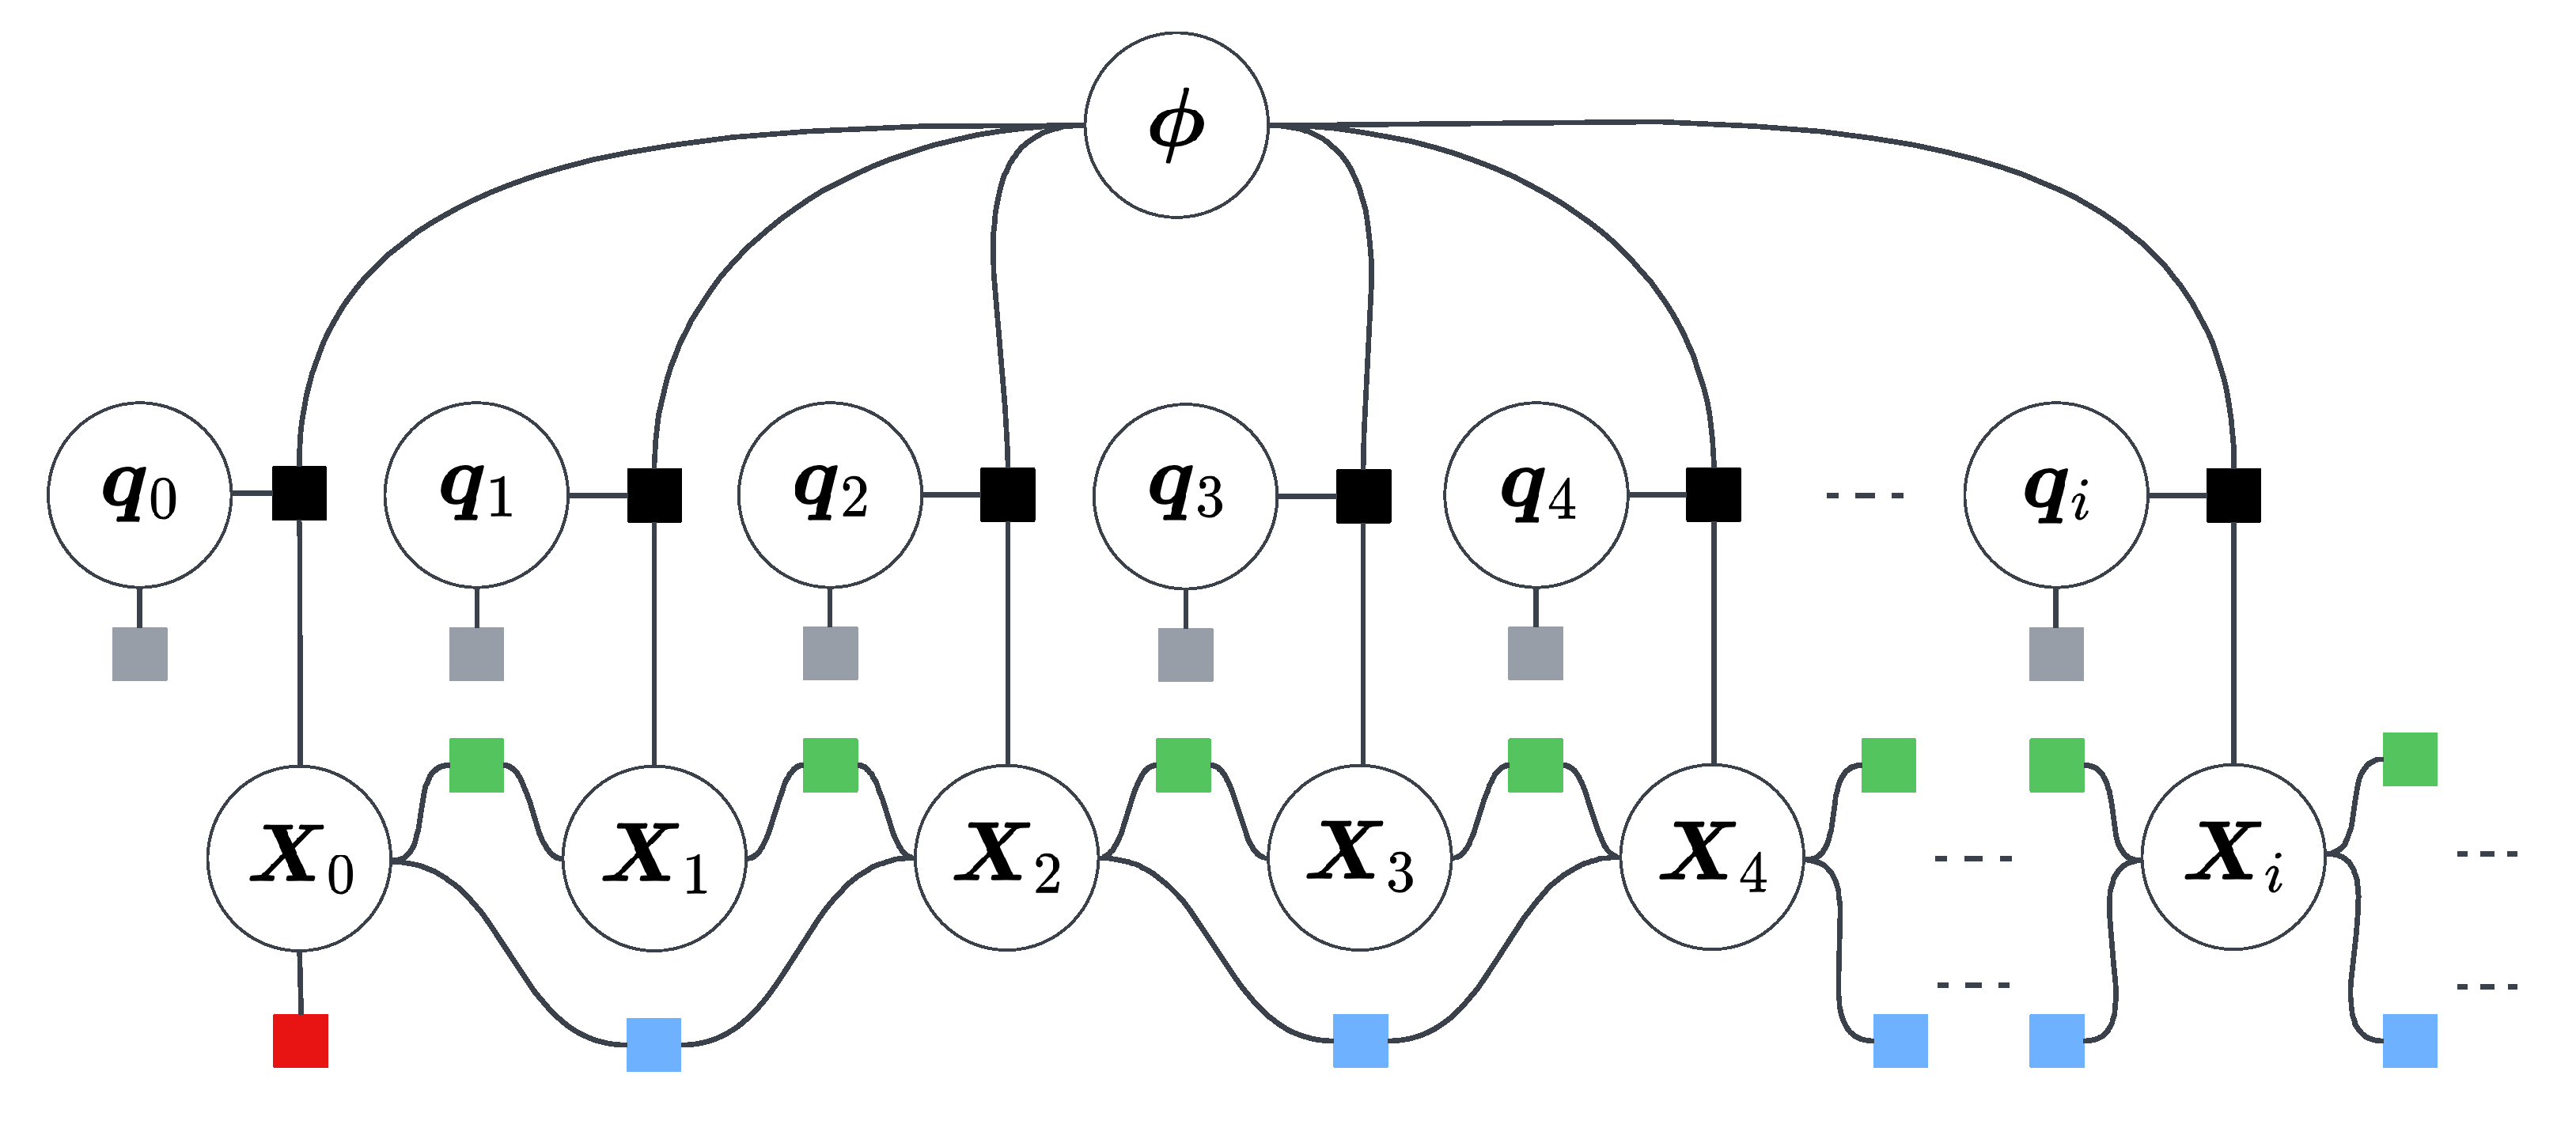
\includegraphics[width=0.7\linewidth]{img/Kinematic_localization_basic}
	\caption{گراف عامل پیشنهادی برای مسئله مکان‌یابی و کالیبراسیون همزمان با پارامتر‌های نامتغیر با زمان}
	\label{fig:kinematiclocalizationbasic}
\end{figure}

فرمول‌بندی سینماتیک بیان‌شده در 
\ref{eq:IK_FK_genral_equations}
می‌تواند طیف وسیعی از ربات‌ها را در بر داشته باشد. به عنوان نمونه، برای روشن‌سازی بهتر مسئله، نمونه موردی ربات
ARASH:ASiST
را باری دیگر در نظر می‌گیریم. شکل
\ref{fig:arashasiststructure}
شمایی از هندسه با ساختاری متوازی‌الاظلاع از این ربات را نشان می‌دهد. پارامترهای سینماتیک این ربات با بردار
$\boldsymbol{\phi} = \{ \alpha, \theta , l_{1234} \} $
مطابق اندازه‌های بیان‌شده بر روی این شکل تعریف می‌شود. همچنین با توجه به مقادیری که بردار مفاصل ربات 
$ \boldsymbol{q}=\{ \phi, \psi, d \} $
دارند، مکان پنجه ربات
$\boldsymbol{X}$
در نقطه دوران از راه دور مشخص شده‌است. با استفاده از این بیان، ساختار سینماتیکی این ربات می تواند به فرمول‌بندی سینماتیک  مستقیم زیر مطابق آنچه در
\cite{hassani2021kinematic}
استخراج شده است، منجر شود:
\begin{equation} \label{eq:arash_asist_fk}
		\begin{aligned}
			\left( \begin{array}{c}
				x \\
				y \\
				z 
			\end{array} \right)
			&=
			\left( \begin{array}{c}
				c_{\theta}(l_{1234} + dc_{\alpha + \psi}) - ds_{\theta}c_{\phi}s_{\alpha + \psi} \\
				s_{\theta}(l_{1234} + dc_{\alpha + \psi}) + d c_{\theta}c_{\phi}s_{\alpha + \psi} \\
				ds_{\phi} s_{\alpha + \psi}
			\end{array} \right)
		\end{aligned}
\end{equation}
که $s$ و $c$ به ترتیب بیانگر توابع 
$\sin(.)$
و
$\cos(.)$
هستند. تفسیر مکان‌یابی و کالیبراسیون سینماتیکی بیان شده در گراف
\ref{fig:kinematiclocalizationbasic}،
استفاده از معادله
\ref{eq:arash_asist_fk}
در عامل‌های بیان شده به عنوان قیود سینماتیکی ربات (عامل‌های سیاه) است. 

\begin{figure}
	\centering
	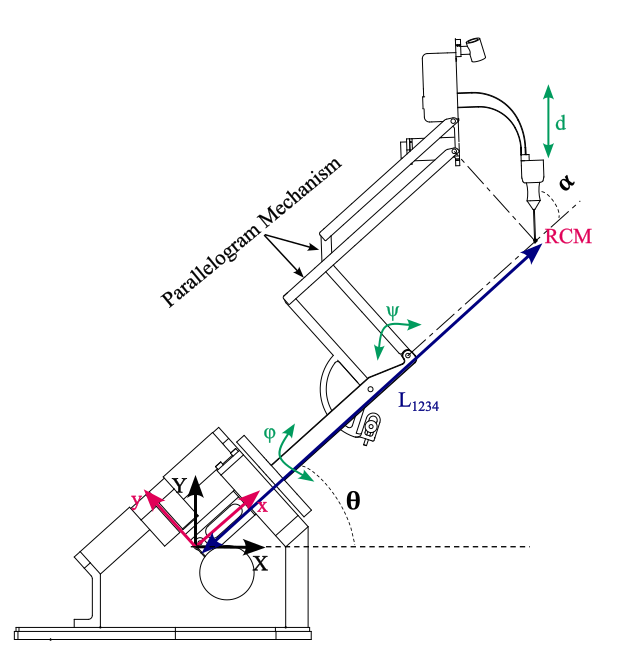
\includegraphics[width=0.5\linewidth]{img/ARASH_ASIST_Structure}
	\caption{نمایی از ساختار ربات ARASH:ASiST}
	\label{fig:arashasiststructure}
\end{figure}

شکل 
\ref{fig:kinematiclocalizationbasicnonstationatyparam}
نشان دهنده گراف قابل استفاده دیگری می باشند که عاری از فرض ثابت بودن پارامترهای کالیبراسیون سینماتیکی بوده و این پارامترها با گذر زمان تغییر می کند و در مسائل زمان واقعی چالش برانگیز هستند. عامل های زرد ایجاد شده در بین پارامترهای کالیبراسیون در زمان های متوالی قیودی هستند که از نوسانات و تغیرات ناگهانی و زیاد این پارامتر های جلوگیری کنند. وجود این قید از آنجایی است که در دنیای واقع انتظار بر تغیر آهسته و منطقی این پارامترهای هندسی می باشد. 
با این بیان صورت گرفته، افزودن قیود متفاوت به مسئله بدون نیاز به تغییر فرمول‌بندی دیگر بخش‌ها قابل انجام خواهد بود. در نهایت، این گراف‌های عامل می‌توانند با استفاده از حل‌کننده‌های افزایشی که کتابخانه GTSAM در اختیار ما قرار می‌دهد، به‌صورت زمان واقعی حل شوند. 

\begin{figure}[b]
	\centering
	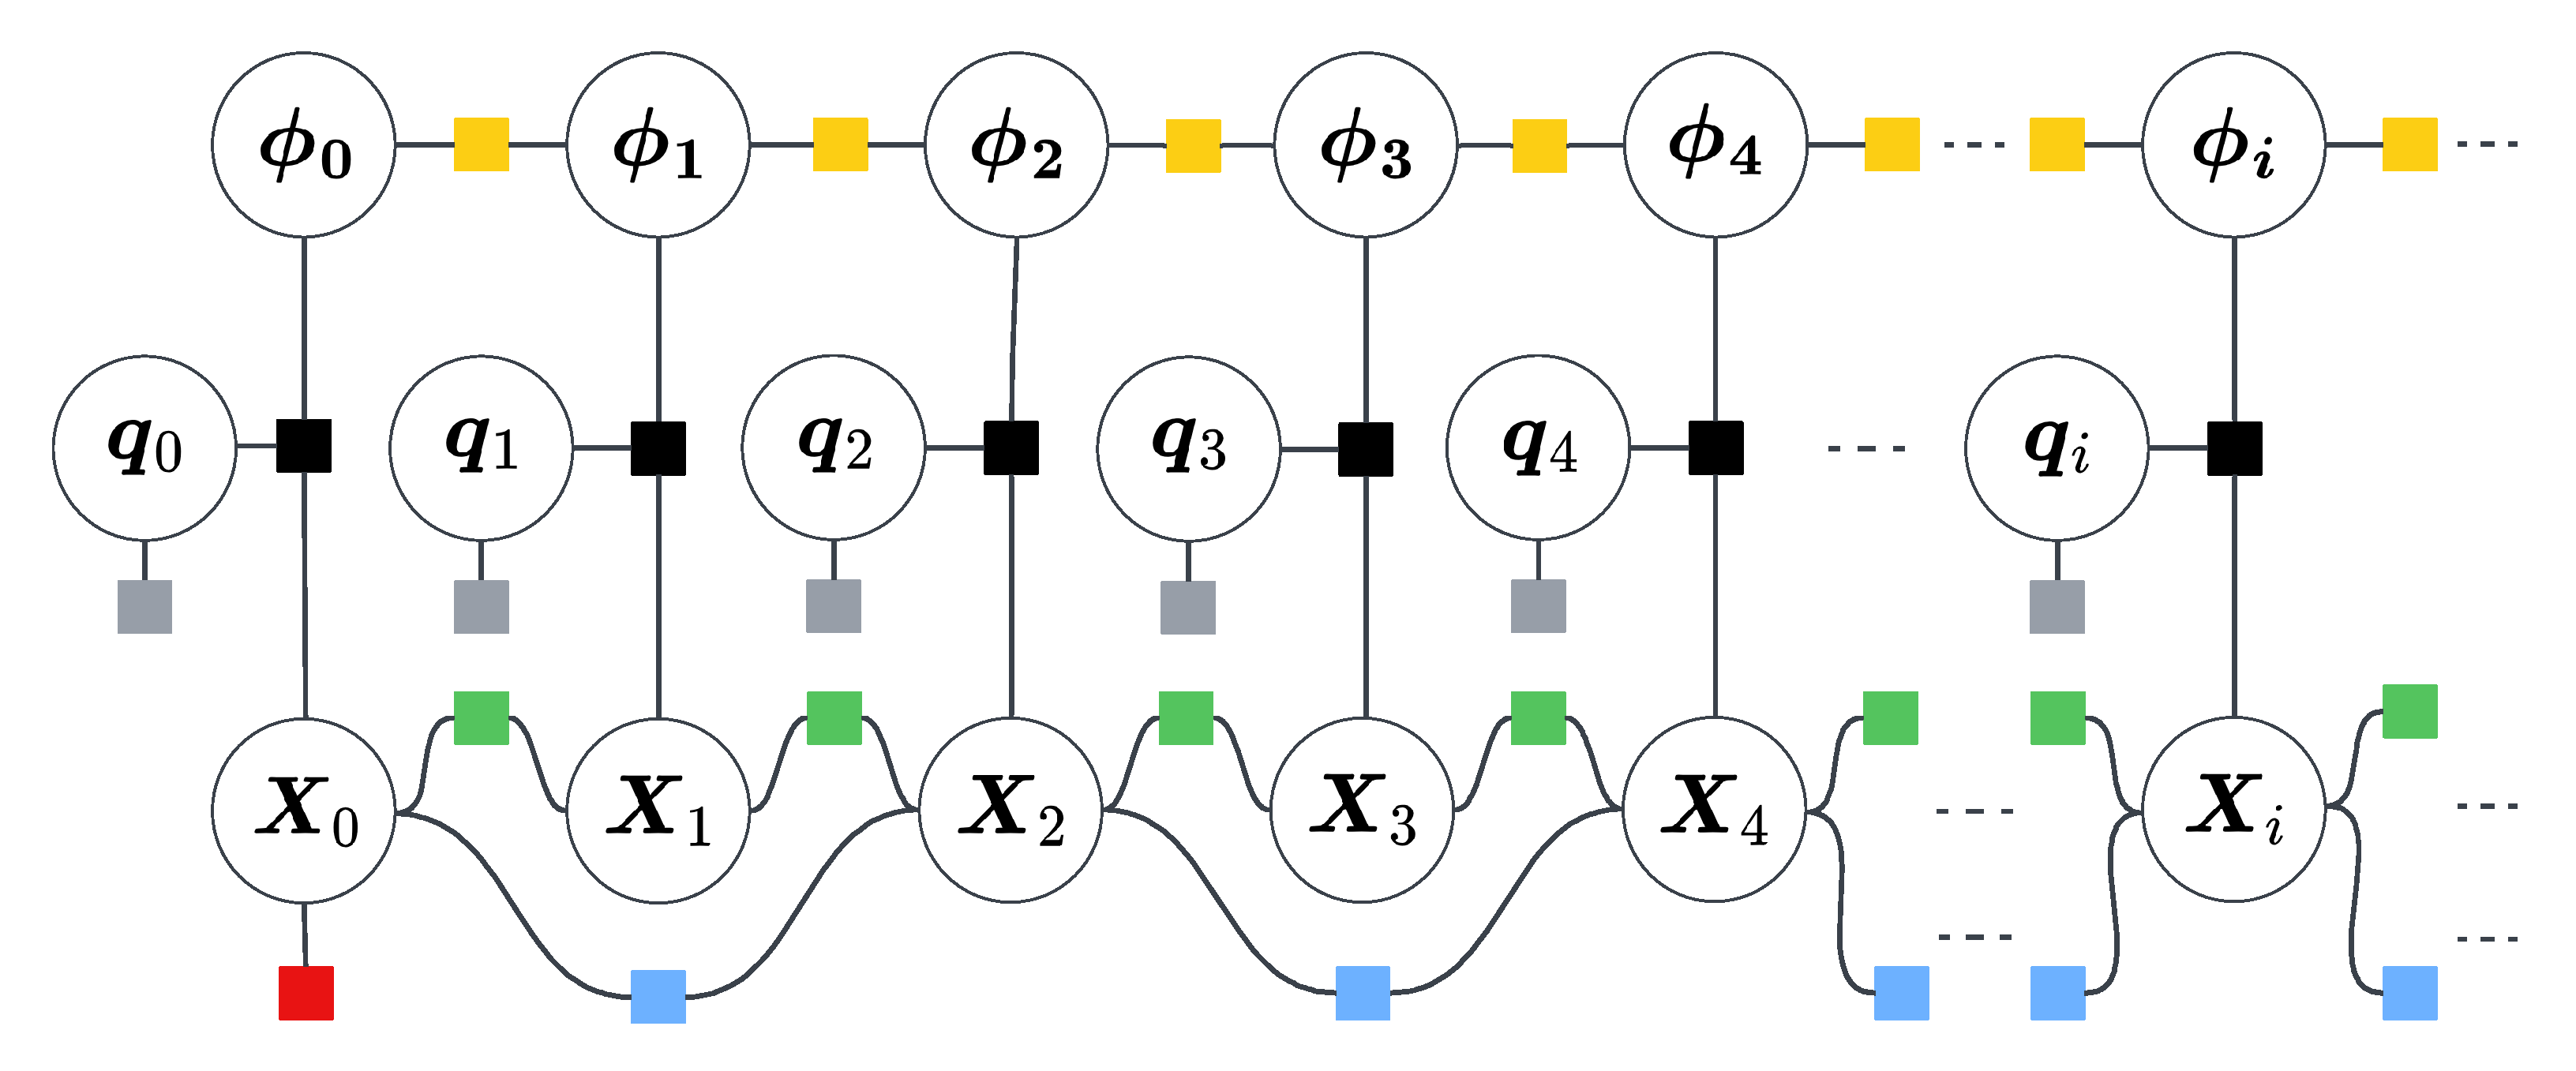
\includegraphics[width=0.7\linewidth]{img/Kinematic_localization_basic_nonstationaty_param}
	\caption{گراف عامل پیشنهادی برای مسئله مکان‌یابی و کالیبراسیون همزمان با پارامتر‌های متغیر با زمان}
	\label{fig:kinematiclocalizationbasicnonstationatyparam}
\end{figure}


\section{نتیجه‌گیری}

در این فصل، رویکرد گراف مبنا برای حل همزمان مسئله کالیبراسیون و مکان‌یابی ربات‌ها مورد بررسی قرار گرفت. این روش با استفاده از گراف‌های عامل، امکان مدیریت بهینه داده‌ها و افزایش دقت محاسبات را فراهم می‌آورد و به راحتی قابل گسترش با قیود و حسگرهای جدید است.

ابتدا مروری بر روش‌های مرسوم مکان‌یابی و کالیبراسیون انجام شد. این روش‌ها، اگرچه ساده و سریع هستند، اما نیاز به بازتعریف مکرر فرمول‌بندی‌ها و خطی‌سازی‌های پیچیده دارند که باعث کاهش دقت و افزایش پیچیدگی محاسبات می‌شود. سپس، رویکردی جدید، بر مبنای گراف‌ها، برای حل این مسئله با توانایی رفع معایب روش‌های مرسوم، مطرح شد.

در معرفی این رویکرد گراف مبنا، مفاهیم پایه‌ای گراف‌های عامل و کاربرد آنها در مدل‌سازی روابط پیچیده بین متغیرها و قیود بیان شد. سپس، با استفاده از معادلات سینماتیکی ربات و داده‌های حسگری، گراف‌های عامل یکپارچه‌ای برای حل مسئله طراحی گردید. این گراف‌ها با توانایی فرمول‌بندی همزمان کالیبراسیون و مکان‌یابی نتایج مطلوبی در بهبود دقت و کارایی ربات را به دست می آورند.



 
 
 
 